\documentclass{beamer}
%~ \usetheme{Hannover}  %% Themenwahl
%~ \usetheme{Bergen}  %% Themenwahl
\usetheme{Berkeley}  %% Themenwahl
\usecolortheme{dove}

\usepackage[utf8]{inputenc}
\usepackage[T1]{fontenc}

\usepackage[english]{babel}

\usepackage{graphicx}
\usepackage{upgreek}
\usepackage{float}
\usepackage{units}
\usepackage{url}

\usepackage{amsmath}
\usepackage{amssymb}
\usepackage{amsfonts}

\usepackage{longtable}

\usepackage{ae}
\usepackage{booktabs}

\usepackage{tikz}
\usetikzlibrary{patterns}

%\abs{Ausdruck} %Betragsstriche, die skalieren - abgekürzt
\newcommand{\abs}[1]{\ensuremath{\left\vert#1\right\vert}}
% und das gleiche füur große Klammern
\newcommand{\brac}[1]{\ensuremath{\left(#1\right)}}
% Erwartungswert skalierend
\newcommand{\avg}[1]{\left< #1 \right>}
% ein nicht kursives d für Ableitungen/Integrale, mit etwas Platz davor, um sich etwas abzusetzten
\newcommand{\de}{\ensuremath{\,\mathrm{d}}}
% Für Einheiten: schreibt sie nicht kursiv und lässt etwas Platz zur Zahl vorher
\newcommand{\eh}[1]{\ensuremath{\,\mathrm{#1}}}
% einfaches Gradzeichen
\newcommand{\gr}{\ensuremath{^{\circ}}}
% Fehlerfortpfanzung
% dy/dz * delta z
\newcommand{\fehler}[2]%
{\ensuremath{\abs{\frac{\partial #1}{\partial #2}}\cdot \Delta #2}}

\title{Ising-Ferromagnet auf Ad-Hoc Netzwerken}
\author{Hendrik Schawe}
\date{\today}

\begin{document}

\maketitle
\frame{\tableofcontents[pausesections]}

\section{Model}
    \subsection{Ising Ferromagnet}
        \begin{frame}{Ising Ferromagnet}
            \begin{equation}
                H = - \sum_{\avg{i,j}}J_{ij}s_{i}s_{j}.
            \end{equation}
            (Ref.\ \cite{Ising1925})
        \end{frame}

    \subsection{Proximity Graphs}
        \begin{frame}{Proximity Graphs}
            \begin{itemize}[<+->]
                \item{ 3 graph types used
                    \begin{itemize}
                        \item Delaunay Triangulation (DT)
                        \item Gabriel Graph (GG)
                        \item Relative Neighborhood Graph (RNG)
                    \end{itemize}
                }
                \item{
                    \begin{equation}
                        DT \supseteq GG \supseteq RNG
                    \end{equation}
                }
            \end{itemize}
        \end{frame}

        \begin{frame}{Delaunay Triangulation}
            \begin{figure}[htbp]
                \centering
                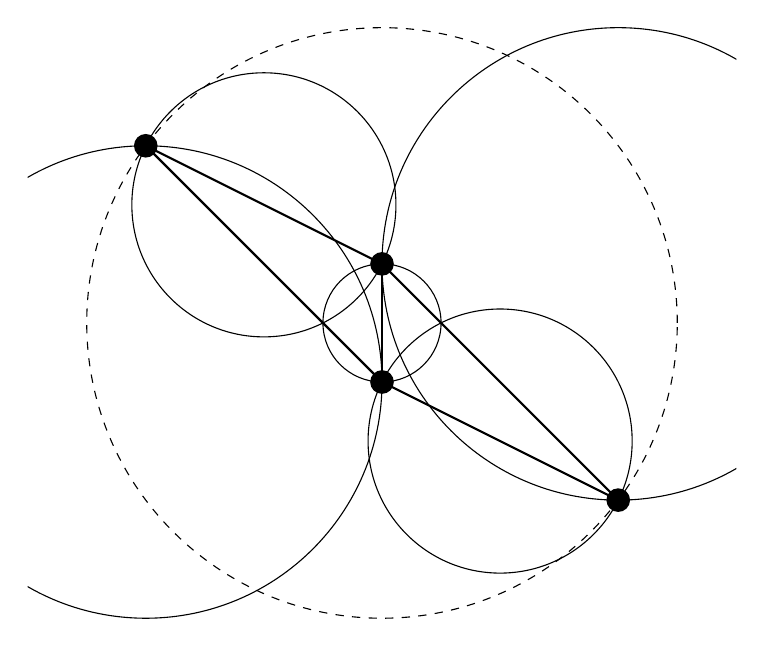
\begin{tikzpicture}[scale=3]
    \clip (-0.5,0) rectangle (2.5,2.5);

    \fill (0, 2  ) circle(0.05);
    \fill (1, 1.5) circle(0.05);
    \fill (1, 1  ) circle(0.05);
    \fill (2, 0.5) circle(0.05);

    \draw[dashed] (1, 1.25)   circle(1.25);
    \draw (2, 1.5)      circle(1);
    \draw (1, 1.25)     circle(0.25);
    \draw (0.5, 1.75)   circle(0.5590);
    \draw (1.5, 0.75)   circle(0.5590);
    \draw (0, 1)        circle(1);

    \draw[thick] (0, 2  ) -- (1, 1.5);
    \draw[thick] (0, 2  ) -- (1, 1  );
    \draw[thick] (1, 1  ) -- (1, 1.5);
    \draw[thick] (1, 1  ) -- (2, 0.5);
    \draw[thick] (1, 1.5) -- (2, 0.5);
\end{tikzpicture}

                \caption
                {
                    Example of a DT.
                }
            \end{figure}
        \end{frame}

        \begin{frame}{Gabriel Graph}
            \begin{columns}[b]
                \begin{column}{5cm}
                    \begin{figure}[htbp]
                        \centering
                        \documentclass{standalone}

\usepackage{tikz}
\usetikzlibrary{arrows}

\begin{document}
    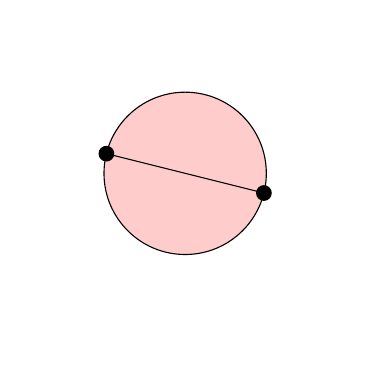
\begin{tikzpicture}
        \clip (-2,2.1) rectangle (2,-2);

        \fill[fill=red!20] (0, 0.25) circle(1.0307764064);
        \draw (0, 0.25) circle(1.0307764064);
        %~ \pattern[pattern color=black!60, pattern=north west lines];


        \fill (-1, 0.5) circle(0.1);
        \fill (1, 0) circle(0.1);
        \draw (1, 0) -- (-1, 0.5);
    \end{tikzpicture}
\end{document}

                        \caption
                        {
                            Lune of a GG.
                        }
                    \end{figure}
                \end{column}
                \begin{column}{5cm}
                    \begin{figure}[htbp]
                        \centering
                        \includegraphics[width=1\textwidth]{images/GG/L12S03.pdf}
                        \caption
                        {
                            GG Example
                        }
                    \end{figure}
                \end{column}
            \end{columns}
        \end{frame}

        \begin{frame}{Relative Neighborhood Graph}
            \begin{columns}[b]
                \begin{column}{5cm}
                    \begin{figure}[htbp]
                        \centering
                        \documentclass{standalone}

\usepackage{tikz}
\usetikzlibrary{arrows}

\begin{document}
    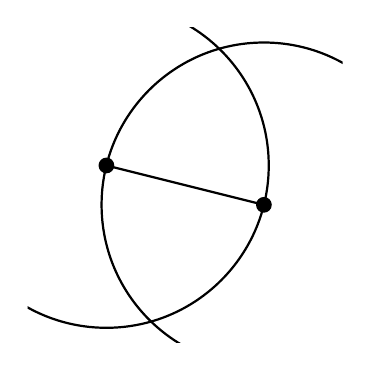
\begin{tikzpicture}
        \clip (-2,2.25) rectangle (2,-1.75);

        \begin{scope}
            \clip (-1, 0.5) circle(2.06155281281);
            \draw (1, 0) circle(2.06155281281);
        \end{scope}

        \draw[thick] (-1, 0.5) circle(2.06155281281);
        \fill (-1, 0.5) circle(0.1);
        \draw[thick] (1, 0) circle(2.06155281281);
        \fill (1, 0) circle(0.1);
        \draw[thick] (1, 0) -- (-1, 0.5);
    \end{tikzpicture}
\end{document}

                        \caption
                        {
                            Lune of a RNG.
                        }
                    \end{figure}
                \end{column}
                \begin{column}{5cm}
                    \begin{figure}[htbp]
                        \centering
                        \includegraphics[width=1\textwidth]{images/RNG/L12S03.pdf}
                        \caption
                        {
                            RNG Example
                        }
                    \end{figure}
                \end{column}
            \end{columns}
        \end{frame}

\section{Methods}
    \subsection{Monte Carlo Simulations}
        \begin{frame}{Monte Carlo Simulations}
            \begin{itemize}[<+->]
                \item generate random states
                \item mesure observables of these states
                \item{ estimate observable \(O\) by
                    \begin{equation}
                        \avg{O} = \frac{1}{Z} \sum_i p_i O_i
                    \end{equation}
                }
            \end{itemize}
            \begin{itemize}[<+->]
                \item But there are states contributing more than others
                \item{ e.g.\ in canonical systems at low \(T\) with
                    \begin{equation}
                        p_{i} = e^{-k_{B}T}
                    \end{equation}
                }
            \end{itemize}
        \end{frame}
        \begin{frame}{Importance Sampling}
            \begin{itemize}[<+->]
                \item{ Markov Chains
                    \begin{itemize}
                        \item Ergodicity
                        \item Detailed Balance
                    \end{itemize}
                }
            \end{itemize}
        \end{frame}


\section{References}
    \begin{frame}[allowframebreaks]
        \bibliography{lit}
        \bibliographystyle{amsplain}
    \end{frame}

\end{document}
